% !TeX encoding = UTF-8
% !TeX program = xelatex
%
% 海南大学研究生学位论文 LaTeX 模板示例主文件
% 文档类选项说明：
%   degree=master|doctor    硕士（默认）/ 博士学位论文
%   anonymous=false|true    正常版（默认）/ 盲审版（自动隐藏作者、导师、学号与致谢）
%   print=false|true        电子提交版（默认）/ 双面装订打印版（前置单面部分自动插空白页）
%   twoside|oneside         双面奇偶页眉页码（默认）/ 单面电子审阅
%   enabstractsize=spec|normal  英文摘要正文按规范 16pt/20pt（默认）或小四 12pt
%   tocdepth=2|3            目录深度：二级（默认，符合 3.7 节）或三级
\documentclass{hainanuthesis}

% ----------------------------------------------------------------------
% 论文基本信息配置
% ----------------------------------------------------------------------
\hainanusetup{
  title        = {基于自适应聚合的联邦学习隐私保护与收敛性分析},
  % subtitle   = {可选副标题},
  title*       = {Privacy-Preserving Adaptive Aggregation and Convergence Analysis in Federated Learning},
  author       = {椰风},
  author*      = {YE Feng},
  supervisor   = {海韵~教授},
  supervisor*  = {HAI Yun},
  student-id   = {202400000001},
  clc          = {TP391},
  secret-level = {}, % 非涉密（公开）论文留空；涉密论文如“秘密（5 年）”
  major        = {计算机科学与技术},
  major*       = {Computer Science and Technology},
  % 填入规范附录 B 中的官方学院全称即可自动映射英文译名；也可手动指定 school* 覆盖
  school       = {计算机科学与技术学院（国际数字影视学院）},
  date         = {2026 年 5 月 20 日},
  date*        = {May, 2026},
  calis-delay  = {none}, % 可选：none | half | one | two
  keywords     = {联邦学习, 自适应聚合, 差分隐私, 收敛性分析, 海南大学},
  keywords*    = {Federated Learning, Adaptive Aggregation, Differential Privacy, Convergence Analysis, Hainan University},
}

% ----------------------------------------------------------------------
% 正文开始
% ----------------------------------------------------------------------
\begin{document}

% 1. 中文封面、英文封面、原创性声明与授权说明（规范 3.10：单面印刷，无页码）
\makecover
\makedeclaration

% 2. 前置部分（大写罗马页码居中，无页眉）
\frontmatter
% !TeX encoding = UTF-8

\begin{cnabstract}
随着数据要素流通与隐私保护法规的日益完善，联邦学习作为一种无需集中原始数据即可实现多方协同建模的分布式机器学习范式，已在智慧医疗、金融风控及自贸港跨境数据协作等场景中展现出重要价值。然而，实际部署环境普遍面临客户端数据非独立同分布（Non-IID）、通信带宽受限以及梯度泄露攻击等关键挑战，导致传统聚合算法收敛缓慢且隐私与效用难以兼顾。

针对上述问题，本文围绕自适应聚合与差分隐私保护机制展开系统研究，主要工作与创新成果如下：（1）构建了基于历史梯度一致性度量的自适应加权聚合框架，有效缓解异构数据分布引发的客户端漂移现象；（2）提出了分阶段动态隐私预算分配策略，在满足 $(\varepsilon, \delta)$-差分隐私理论保障的前提下显著降低了噪声注入对模型精度的损害；（3）给出了非凸目标函数下的严格收敛上界证明，并在多个公开基准数据集上验证了所提方法的有效性与通信效率。

实验结果表明，在高度异构的数据划分与同等隐私预算约束下，本文方法相较经典基准算法将测试准确率提升了 3.8\% 至 6.2\%，同时将达到目标精度所需的通信轮次减少了约 31\%，为面向多主体协作场景的可信联邦学习系统落地提供了理论支撑与工程参考。
\end{cnabstract}

\begin{enabstract}
With the rapid advancement of data governance regulations and privacy protection requirements, federated learning has emerged as a promising distributed machine learning paradigm that enables collaborative model training without centralizing raw private data. Nevertheless, practical deployments frequently suffer from non-independent and identically distributed (Non-IID) client data, constrained communication bandwidth, and gradient inversion attacks, resulting in degraded convergence speed and unfavorable privacy-utility trade-offs.

To address these challenges, this thesis investigates privacy-preserving adaptive aggregation and its theoretical convergence properties. First, an adaptive weighted aggregation mechanism driven by historical gradient consistency is formulated to mitigate client drift under severe statistical heterogeneity. Second, a stage-wise dynamic privacy budget allocation scheme is designed to preserve $(\varepsilon, \delta)$-differential privacy while minimizing accuracy degradation. Third, a tight non-convex convergence upper bound is established theoretically and validated empirically across representative benchmark datasets.

Extensive experimental results demonstrate that the proposed approach improves test accuracy by 3.8\% to 6.2\% over standard baselines under identical privacy budgets while reducing communication rounds by approximately 31\%.
\end{enabstract}

\maketoc
\makelistoffigures
\makelistoftables
% !TeX encoding = UTF-8

\begin{denotation}[主要符号表]
\noindent
\begin{tabularx}{\textwidth}{@{}>{\centering\arraybackslash}p{3.0cm} X@{}}
  \toprule
  符号 / 缩略词 & 含义说明 \\
  \midrule
  $\mathcal{D}_k$ & 第 $k$ 个客户端所持有的本地训练数据集 \\
  $K$             & 参与联邦协同训练的客户端总数 \\
  $\mathbf{w}^t$  & 第 $t$ 轮通信后的全局模型参数向量 \\
  $\eta_t$        & 第 $t$ 轮本地随机梯度下降的学习率 \\
  $\varepsilon, \delta$ & 差分隐私预算参数与松弛概率 \\
  Non-IID         & 非独立同分布（Non-Independent and Identically Distributed） \\
  SGD             & 随机梯度下降（Stochastic Gradient Descent） \\
  \bottomrule
\end{tabularx}
\end{denotation}


% 3. 主体部分（阿拉伯数字页码：奇右偶左；双面页眉：奇“海南大学硕士/博士学位论文”，偶一级章标题）
\mainmatter
% !TeX encoding = UTF-8

\chapter{绪论}

\section{研究背景与意义}

近年来，人工智能与大数据技术在医疗健康、金融风控与智慧城市等领域取得了突破性进展。然而，随着《中华人民共和国数据安全法》《中华人民共和国个人信息保护法》等法律法规相继实施，数据孤岛与隐私合规之间的矛盾日益凸显。传统集中式机器学习范式需要将各参与方的原始数据汇聚至中心服务器统一训练，不仅带来高昂的传输与存储开销，还存在严重的隐私泄露隐患。

为应对上述挑战，联邦学习（Federated Learning，FL）作为一种新兴的分布式协同训练范式应运而生\cite{mcmahan2017fedavg}。在联邦学习框架中，原始训练样本始终保留在本地客户端，参与方仅周期性地与中心服务器交互模型参数或梯度更新。由文献\citeinline{kairouz2021advances}可知，联邦学习在数据分布高度异构（Non-IID）与恶意推理攻击并存的开放环境下，依然面临收敛速度慢、通信代价高与隐私效用权衡困难等核心瓶颈。

\section{国内外研究现状}

\subsection{联邦聚合优化研究进展}

经典的联邦平均算法（FedAvg）通过在客户端执行多步本地随机梯度下降并按样本量加权平均，有效降低了通信频率\cite{mcmahan2017fedavg}。但在非独立同分布数据场景下，本地目标函数与全局目标函数之间的偏差会诱发显著的客户端漂移现象。在工程优化与文献著录实践中，严谨的格式规范与统计建模方法同样至关重要\cite{chenjianjun2001,gbt7714_2015}。

\subsubsection{非独立同分布数据缓解机制}

面向统计异构问题，现有研究主要沿两条技术路线展开：其一是在本地优化目标中引入正则化约束或控制变量，以校正本地梯度方向\footnote{此处演示规范 1.9 节所规定的页下“脚注”注释方式，适用于对正文术语或未公开发表资料的补充说明。}；其二是在服务器端设计基于梯度相似度或历史动量的自适应聚合策略。

\subsubsection{差分隐私与通信压缩协同设计}

已有研究表明，单纯传输梯度信息仍可能遭受梯度反演攻击并还原原始样本\cite{mahuan2011}。结合差分隐私噪声注入与梯度稀疏化能够兼顾安全性与带宽约束，相关专利与标准规范也提供了重要工程借鉴\cite{jiangxizhou1989,dublincore2012}。

\section{本文主要研究内容与结构安排}

本文严格遵循《海南大学研究生学位论文撰写规范（修订）》（海大党政办〔2023〕47 号）的结构要求，全文章节安排如下：第 1 章介绍研究背景与国内外现状；第 2 章阐述自适应聚合框架、数学公式推导与三线表及跨页续表排版示例；第 3 章展示实验配置、曲线图与对比结果分析；第 4 章总结全文主要结论并展望未来研究方向。

% !TeX encoding = UTF-8

\chapter{理论基础与方法设计}

\section{问题建模与数学表达式}

考虑包含 $K$ 个客户端的横向联邦学习系统，第 $k$ 个客户端持有本地私有数据集 $\mathcal{D}_k$，样本规模为 $n_k = |\mathcal{D}_k|$，总样本数为 $N = \sum_{k=1}^{K} n_k$。系统的全局经验风险最小化目标如式~(\ref{eq:global-obj}) 所示：
\begin{equation}
  \min_{\mathbf{w} \in \mathbb{R}^{d}} F(\mathbf{w})
  = \sum_{k=1}^{K} p_k F_k(\mathbf{w}),
  \quad
  F_k(\mathbf{w}) = \frac{1}{n_k} \sum_{\xi \in \mathcal{D}_k} \ell(\mathbf{w}; \xi),
  \label{eq:global-obj}
\end{equation}
其中，$p_k = n_k / N$ 表示客户端 $k$ 的基准权重，$\ell(\mathbf{w}; \xi)$ 为样本 $\xi$ 上的损失函数。

在第 $t$ 轮通信中，服务器聚合经裁剪与高斯噪声扰动后的客户端模型增量 $\tilde{\Delta}_k^t$，全局参数更新规则可表述为：
\begin{equation}
  \mathbf{w}^{t+1}
  = \mathbf{w}^t + \sum_{k \in \mathcal{S}_t} \alpha_k^t \tilde{\Delta}_k^t
  + \mathcal{N}\!\left(\mathbf{0}, \sigma_t^2 C^2 \mathbf{I}_d\right),
  \label{eq:dp-update}
\end{equation}
其中，$\alpha_k^t$ 为基于历史梯度余弦一致性动态计算的自适应聚合权重，$\sigma_t$ 为第 $t$ 轮隐私噪声尺度，$C$ 为裁剪阈值。

\begin{theorem}[非凸目标收敛上界]
  若各客户端局部目标函数 $F_k$ 满足 $L$-光滑条件且随机梯度方差有界（上界为 $\sigma_g^2$），则当学习率满足 $\eta_t \le \frac{1}{4 L E}$ 时，经过 $T$ 轮通信后算法满足：
  \begin{equation}
    \frac{1}{T} \sum_{t=0}^{T-1} \mathbb{E}\!\left[\|\nabla F(\mathbf{w}^t)\|^2\right]
    \le \mathcal{O}\!\left(\frac{1}{\sqrt{K E T}}\right)
    + \mathcal{O}\!\left(\frac{d \sigma^2}{T}\right).
    \label{eq:conv-bound}
  \end{equation}
\end{theorem}

\begin{proof}
  利用 $L$-光滑性对 $F(\mathbf{w}^{t+1}) - F(\mathbf{w}^t)$ 进行二阶泰勒展开，结合噪声项的零均值独立性并在 $t = 0, \dots, T-1$ 上累加取期望即可得证，详细推导见附录~A。
\end{proof}

\section{核心参数与三线表示例}

按照规范 2.4.2 节要求，表中参数应标明量和单位的符号，表序与表题居中排于表的上方，推荐使用国际通行的三线表。本文关键超参数配置见表~\ref{tab:hyperparams}。

\begin{table}[htbp]
  \centering
  \caption{联邦学习与隐私保护关键超参数设置}
  \label{tab:hyperparams}
  \begin{tabular}{@{}l c l@{}}
    \toprule
    参数名称 & 符号与取值 & 说明 \\
    \midrule
    客户端总数 & $K = 100$ & 每轮随机采样率 $q = 0.1$ \\
    本地训练轮数 & $E = 5\,\mathrm{epochs}$ & 批大小 $B = 64$ \\
    初始学习率 & $\eta_0 = 0.01$ & 余弦退火调度 \\
    梯度裁剪阈值 & $C = 1.0$ & 逐客户端 $\ell_2$ 范数裁剪 \\
    隐私预算 & $\varepsilon \in \{2.0, 4.0, 8.0\}$ & 松弛项 $\delta = 10^{-5}$ \\
    \bottomrule
  \end{tabular}
\end{table}

\section{跨页续表示范}

当表格行数较多需要跨页排版时，规范 2.4.2 节要求在续表上方居中注明“续表”并重复排出表题。下方的表~\ref{tab:long-demo} 演示了使用 \texttt{longtable} 实现标准跨页三线表的写法。

\begin{longtable}{@{}c l c c@{}}
  \caption{不同数据异构程度下的通信与精度记录}
  \label{tab:long-demo} \\
  \toprule
  实验编号 & 异构划分参数（Dirichlet $\alpha$） & 通信轮次 $T$ / 轮 & 测试准确率 / \% \\
  \midrule
  \endfirsthead

  \multicolumn{4}{c}{\zihao{5}\songti 续表} \\
  \caption*{表~\thetable\quad 不同数据异构程度下的通信与精度记录} \\
  \toprule
  实验编号 & 异构划分参数（Dirichlet $\alpha$） & 通信轮次 $T$ / 轮 & 测试准确率 / \% \\
  \midrule
  \endhead

  \bottomrule
  \endfoot

  \bottomrule
  \endlastfoot

  E-01 & $\alpha = 0.10$（极度异构） & 100 & 74.2 \\
  E-02 & $\alpha = 0.10$（极度异构） & 150 & 78.6 \\
  E-03 & $\alpha = 0.30$（高度异构） & 100 & 80.5 \\
  E-04 & $\alpha = 0.30$（高度异构） & 150 & 83.9 \\
  E-05 & $\alpha = 0.50$（中度异构） & 100 & 84.1 \\
  E-06 & $\alpha = 0.50$（中度异构） & 150 & 86.7 \\
  E-07 & $\alpha = 1.00$（轻度异构） & 100 & 86.4 \\
  E-08 & $\alpha = 1.00$（轻度异构） & 150 & 88.2 \\
\end{longtable}

% !TeX encoding = UTF-8

\chapter{实验设计与结果分析}

\section{实验环境与基准方法}

本节在公开图像分类基准数据集上对所提自适应聚合方法进行对比验证，主要对比方法包括经典联邦平均算法 FedAvg\cite{mcmahan2017fedavg} 及固定噪声尺度差分隐私基线 DP-FedAvg。

\section{收敛性能曲线分析}

按照规范 2.4.1 节要求，插图一般随文编排、先见文字后见图；图序与图题居中排于图的下方，曲线图纵横坐标应标注“量、标准规定符号、单位”，且不同曲线采用不同形状标识符区分。如图~\ref{fig:conv-curve} 所示，本文方法在前期通信轮次中即展现出更快的收敛速率与更平滑的泛化曲线。

\begin{figure}[htbp]
  \centering
  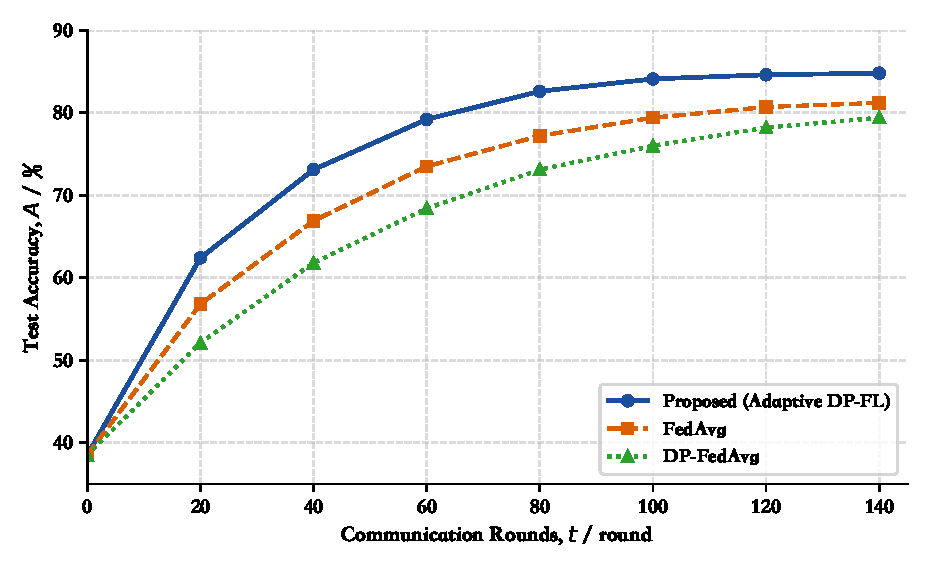
\includegraphics[width=0.78\textwidth]{figures/demo-curve.pdf}
  \caption{不同聚合算法在异构数据下的测试准确率收敛曲线}
  \label{fig:conv-curve}
\end{figure}

图~\ref{fig:subfigs} 展示了双子图并排排版示例，图序与子图编号均自动匹配五号宋体规范要求。

\begin{figure}[htbp]
  \centering
  \begin{subfigure}[b]{0.47\textwidth}
    \centering
    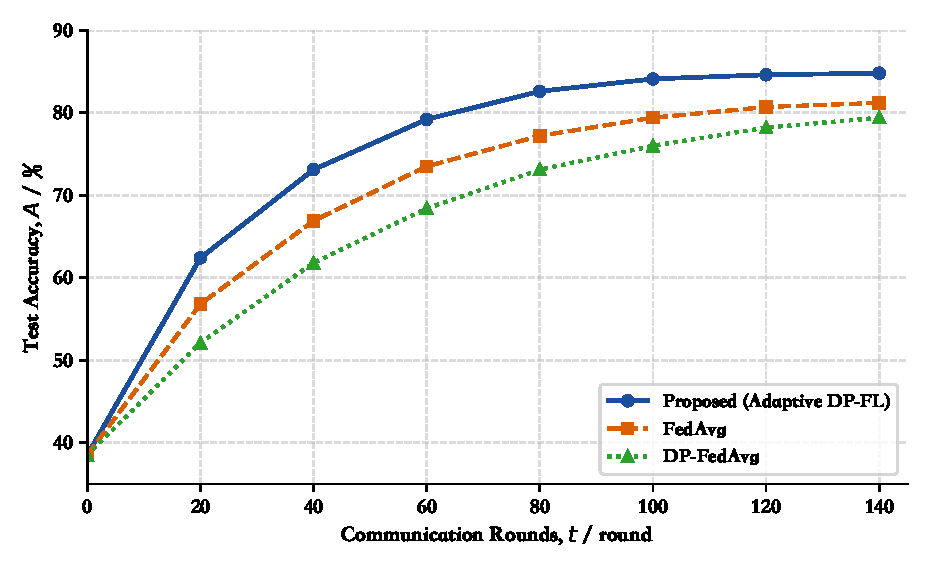
\includegraphics[width=\textwidth]{figures/demo-curve.pdf}
    \caption{隐私预算 $\varepsilon = 4.0$}
    \label{fig:sub-a}
  \end{subfigure}
  \hfill
  \begin{subfigure}[b]{0.47\textwidth}
    \centering
    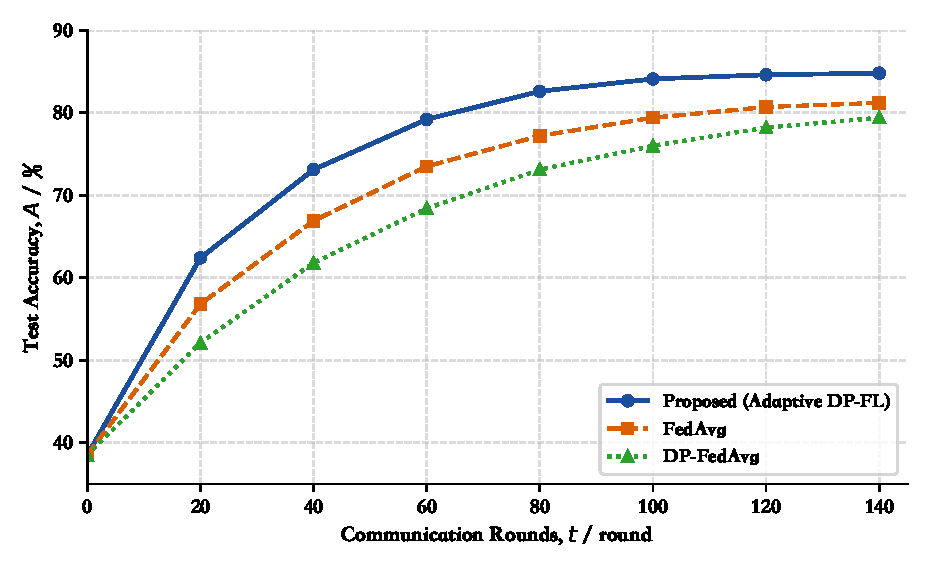
\includegraphics[width=\textwidth]{figures/demo-curve.pdf}
    \caption{隐私预算 $\varepsilon = 8.0$}
    \label{fig:sub-b}
  \end{subfigure}
  \caption{不同隐私预算约束下的算法性能对比}
  \label{fig:subfigs}
\end{figure}

\section{消融实验与讨论}

表~\ref{tab:ablation} 汇总了各核心模块对最终测试准确率与通信轮次的贡献。移除动态隐私预算分配或梯度一致性加权均会导致模型准确率明显下降，表明两个模块在非独立同分布与隐私噪声耦合场景下具有良好互补性\cite{chendengyuan2000}。

\begin{table}[htbp]
  \centering
  \caption{核心模块消融实验结果对比}
  \label{tab:ablation}
  \begin{tabular}{@{}l c c c@{}}
    \toprule
    方法变体 & 最终准确率 / \% & 达标通信轮次 / 轮 & 相对增益 / \% \\
    \midrule
    DP-FedAvg（基线） & 79.4 & 145 & — \\
    + 梯度一致性自适应加权 & 82.6 & 112 & +3.2 \\
    + 分阶段动态隐私预算 & 81.9 & 118 & +2.5 \\
    完整方法（本文） & \textbf{84.8} & \textbf{98} & \textbf{+5.4} \\
    \bottomrule
  \end{tabular}
\end{table}

% !TeX encoding = UTF-8

\chapter{结论与展望}

\section{全文总结}

本文针对联邦学习在实际部署中面临的数据统计异构与隐私效用失衡难题，设计了基于梯度一致性度量的自适应聚合框架与分阶段动态隐私预算分配机制，并完成了非凸收敛理论证明与系统实验验证。主要结论如下：
\begin{enumerate}[label=（\arabic*）, leftmargin=2\ccwd, itemsep=2pt]
  \item 引入历史梯度余弦一致性权重能够显著抑制客户端漂移，在不增加额外通信负载的前提下加快收敛速度；
  \item 分阶段动态噪声调度机制将更多隐私预算分配至模型精调阶段，有效平衡了 $(\varepsilon, \delta)$-差分隐私保障与模型泛化精度；
  \item 在多种异构强度与隐私预算配置下，所提方法在测试准确率与通信效率两项指标上均稳定优于对比基线。
\end{enumerate}

\section{研究局限与未来展望}

尽管本文工作取得了预期成效，但在大规模跨设备异步通信以及抵御拜占庭恶意投毒攻击等方面仍有进一步拓展空间。未来工作将探索面向异步联邦环境的自适应隐私会计方法，并结合硬件可信执行环境提升系统整体安全性。


% 4. 参考文献（GB/T 7714-2015 顺序编码制）
\makebibliography{bib/references}

% 5. 附录（编号自动切换为：附录 A、图 A1、表 A1、(A1)）
\appendix
% !TeX encoding = UTF-8

\chapter{核心定理推导补充}

本附录演示规范 1.11 节要求的附录格式：附录编号与附录标题各占一行并居中排列；附录中的公式、图和表分别自动编号为 \texttt{(A1)}、\texttt{图 A1}、\texttt{表 A1}。

在满足 $L$-光滑性假设条件下，局部更新误差的一步递推不等式可写为：
\begin{equation}
  \mathbb{E}\!\left[\|\mathbf{w}_k^{t, r} - \mathbf{w}^t\|^2\right]
  \le 5 E \eta_t^2 \left(\sigma_g^2 + 6 E \zeta^2\right),
  \label{eq:appendix-lemma}
\end{equation}
式~(\ref{eq:appendix-lemma}) 的编号自动采用 \texttt{(A1)} 形式。

\begin{table}[htbp]
  \centering
  \caption{附录补充实验数据集统计特征}
  \label{tab:appendix-dataset}
  \begin{tabular}{@{}l c c c@{}}
    \toprule
    数据集 & 类别数 & 训练样本量 / 条 & 测试样本量 / 条 \\
    \midrule
    Fashion-MNIST & 10 & 60\,000 & 10\,000 \\
    CIFAR-10      & 10 & 50\,000 & 10\,000 \\
    \bottomrule
  \end{tabular}
\end{table}

\begin{figure}[htbp]
  \centering
  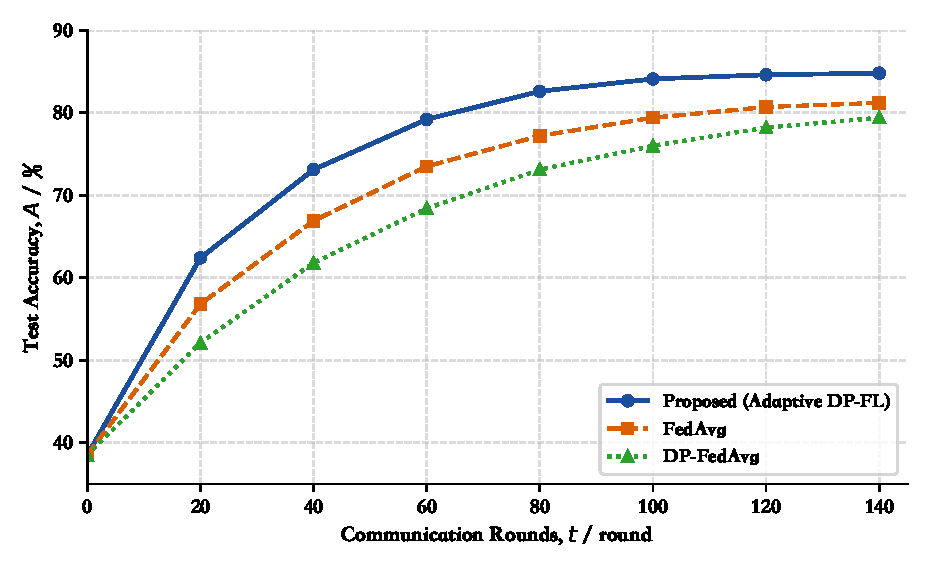
\includegraphics[width=0.68\textwidth]{figures/demo-curve.pdf}
  \caption{附录补充收敛稳定性验证曲线}
  \label{fig:appendix-fig}
\end{figure}


% 6. 结尾部分：攻读学位期间取得的成果与致谢
\backmatter
% !TeX encoding = UTF-8

\begin{achievements}
\noindent\textbf{一、已发表及录用学术论文}
\begin{enumerate}[label={[\arabic*]}, leftmargin=2.2em, itemsep=4pt]
  \item 椰风, 海韵. 面向异构联邦学习的自适应差分隐私聚合方法研究[J]. 计算机学报, 2026, 49(3): 112-125.（EI 检索，第一作者）
  \item YE F, HAI Y. Adaptive Privacy-Preserving Aggregation for Non-IID Federated Learning[C]//Proceedings of the IEEE International Conference on Distributed Computing Systems. Piscataway: IEEE, 2025: 204-213.（CCF-B 类会议，第一作者）
\end{enumerate}

\vspace{0.6\baselineskip}
\noindent\textbf{二、申请发明专利与科研项目}
\begin{enumerate}[label={[\arabic*]}, leftmargin=2.2em, itemsep=4pt]
  \item 海韵, 椰风. 一种基于梯度一致性的联邦学习隐私保护聚合方法及系统: 中国, CN202510000001.X[P]. 2025-11-15.（实审阶段）
  \item 国家自然科学基金面上项目（编号：624XXXXX），“可信分布式协同学习理论与关键技术研究”，2025—2028，主要参与人。
\end{enumerate}
\end{achievements}

% !TeX encoding = UTF-8

\begin{acknowledgements}
时光荏苒，转眼间在海南大学海甸校区的求学生涯即将画上句号。回望这几年的科研探索与成长历程，谨向所有给予我悉心指导、热情帮助与真诚鼓励的师长、同窗及家人致以最诚挚的谢意。

首先，衷心感谢我的导师海韵教授。从课题选题、理论推导、实验验证到论文成稿的每一个环节，海老师都倾注了大量心血。导师严谨求实的治学态度、敏锐深邃的学术洞察力以及宽厚仁爱的育人风范，将使我终身受益。

感谢学院各位授课老师和答辩委员会专家在开题、中期及预答辩阶段提出的宝贵意见；感谢实验室的师兄师姐与同门挚友在日常学术研讨与代码调试中的无私相助。

最后，感谢我的父母与家人多年来默默的支持与包容，正是你们的关爱给予了我不断前行的力量。祝愿海南大学各项事业蒸蒸日上！
\end{acknowledgements}


% 如需单独生成书脊页面，取消下一行注释
% \makespine

\end{document}
